% !TEX root = ../../main.tex
\section{Classic diffusion theory in population genetics}

The pioneers of the modern-synthesis of evolution established solid foundations
for how to understand the different forces at play that shape the structure of
evolving populations. But combining all of these forces into a single
description remained challenging. In other words, describing the outcome of an
evolutionary process that combined deterministic processes such as selection
and mutation with the stochasticity of evolution presented a challenging
mathematical puzzle. The first attempt to put everything together came from
Sewall Wright himself, but the achievement of formalizing the theory is often
associated with a remarkable Japanese population genetics by the name of Motoo
Kimura.

Kimura jump to fame when in 1968 he presented his \textit{Neutral theory of
molecular evolution}. In here Kimura argued that associating every biological
aspect to the outcome of a selection-driven process was too much of a naive
picture. We previously mentioned that Wright thought about genetic drift as an
important component of the evolutionary process, but in this 1968 paper Kimura
argued that it was \textit{the} dominant force in evolution.

But what really brings us here to study part of Kimura's scientific legacy is
his use of diffusion equations in the context of population genetics. What we
know now as Kimura's diffusion theory is nothing else than the application of
the mathematical tools developed for the study of physical diffusion of
particles to evolving populations. Diffusion is one of several transcendent
concepts in physics that demonstrate the power of universal concepts. The same
equation that describes how the concentration of a chemical species changes as
a function of space and time is used to describe how the temperature profile of
an object changes as a function of space and time as well. Furthermore, as we
will study in this section, the same mathematical language can describe
diffusion on an abstract space of allele frequency. So as Joe Blitzstein likes
to say: ``nouns change, but the verbs remain the same.''

The mathematical language to study diffusion theory, as with many other field
of science is the language of probability theory. As Jaynes' famous book title
suggested, \textit{probability theory is the logic of science}. It is through
this formal language that we can assess how likely are specific events to
happen. For example, later on we'll see that within the framework of diffusion
theory is possible to ask what is the probability of an allele being fixed in
the population given the evolutionary forces acting on it. In particular we are
interested in a type of probability object known as a Markov process that we
will now define.

\subsection{Markov processes}
Of particular interested for our endeavor are the specific mathematical objects
known as Markov processes. The Markovian property - named after Andrey Markov,
a famous Russian mathematician from the XIX century - can be stated as follows:
A Markov process is a type of stochastic process for which the transition
states only depends on the current state.

To gain intuition for what this means imagine we are measuring a variable $x$
over time such that we have a bunch of pairs of the form $(x_1, t_1), (x_2,
t_2), (x_3, t_3), \ldots (x_{n+1}, t_{n+1})$. For a Markov process, the
probability of ending at state $x_{n+1}$ at time $t_{n+1}$ given all the
previous visited states is of the form
\begin{equation}
  P(x_{n+1}, t_{n+1} \mid x_1, t_1; x_2, t_2; \ldots; x_n, t_n) =
  P(x_{n+1}, t_{n+1} \mid x_n, t_n).
  \label{eq_chapman_kolmogorov}
\end{equation}
In other words, knowing the entire history of variable $x$ as it evolves over
time does not help us predict the next time step. All we need to know is the
last position. Markov processes are usually called memoryless stochastic
process because of this property that the process doesn't remember the full
trajectory when it ``decides'' where to move in the next step. Assuming a
Markovian process is arguably one of the most widely used assumptions in all of
science; from chemical reactions, to brownian motion of a particle, to our
particular case of interest of allele frequencies changing over time.

In the classic formulation of diffusion theory we are concerned with a
particular type of Markov processes. Diffusion theory works in the limit of
large populations where we can assume that the frequency of a particular allele
rather than being a discrete entity that changes in factors of $1 / N$ where
$N$ is the number of organisms, is a continuous value in the range between 0
and 1. We also assume that we can compute changes in this frequency in
continuous time. That means that both $f$ the frequency of an allele, and $t$
the time are continuous variables. Therefore we are interested in a type of
Markov processes that go by the creative name of continuous-time
continuous-state Markov processes. We will now state a very important equation
for this type of Markovian processes known as the Chapman-Kolmogorov equation.

\subsubsection{Chapman-Kolmogorov equation} \label{sec_chapman_kolmogorov}

The Chapman-Kolmogorov equation is an important property of continuous-time
continuous-state Markov processes that we will use for many of our derivations
in the coming sections. The equation is stated as follows: For three time points
$t_1 < t_2 < t_3$ for which we measured a stochastic variable $x$ we have that
\begin{equation}
  P(x_3, t_3 \mid x_1, t_1) = \int dx_2\; P(x_3, t_3 \mid x_2, t_2)
                                          P(x_2, t_2 \mid x_1, t_1),
\end{equation}
where the integral is taken over the domain of values that the random variable
$x$ can take. In other words, to calculate the transition probability between
$x_1$ and $x_3$ with an intermediary step $x_2$, we must add (integrate for
continuous variables) all possible values that $x_2$ can take. This concept is
schematically represented in \fref{fig_chapman_kolmogorov}

\begin{figure}[h!]
	\centering 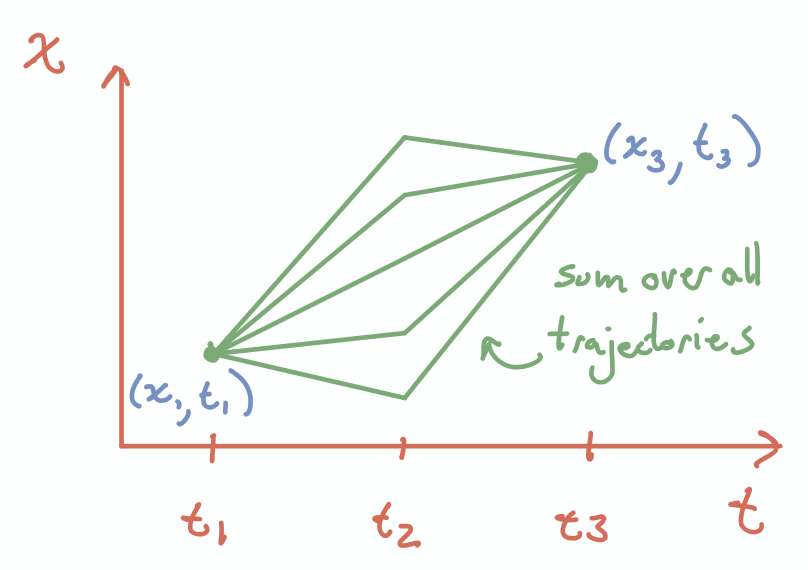
\includegraphics[width=0.5\textwidth]
  {../fig/classic_diffusion/03_02_01_chapman_kolmogorov.png}
	\caption{\textbf{Schematic of the Chapman-Kolmogorov equation}. The
  Chapman-Kolmogorov equation is a statement about the transition between two
  points $x_1$ and $x_3$, adding all possible intermediary steps $x_2$.}
  \label{fig_chapman_kolmogorov}
\end{figure}

In the coming section we will use the Chapman-Kolmogorov equation to derive the
so-called continuous master equation. This will be the foundation from which we
will get to the main results of diffusion theory. But before jumping into such
matter we need to introduce a specific subtype of Markov processes.

\subsubsection{Stationary Markov Process}\label{sec_stationary_process}

When thinking about evolution we often summon the concept of a mapping between
genotype (sequence level description) to phenotype (observable characteristic)
to fitness (reproductive success). This concept goes by several names, but in
1932 Sewall Wright attempted to formalize this idea as \textit{adaptive
landscapes}. The phenotype itself can be a function of the genotype and the
environmental state that can itself change over time either deterministically
or stochastically. Therefore the idea of a ``landscape'' is not necessarily the
best description. Some authors have discussed concepts such as \textit{fitness
seascapes} when the environment evolves over time independently of the organism
or \textit{fitness snowscapes} when there is a direct interaction between
organisms modifying the environment, and the environment modifying the
organisms.

For simplicity we usually work with fixed fitness landscapes. This
approximation is valid under certain time-scale regimes. For example, if the
environment does change over time, but it does it on a time-scale much longer
than what it takes for organisms to adapt, then we can pretend for our
calculations that the environment is fixed, simplifying the math enormously.
For this particular case where the mapping all the way from genotype to fitness
is not a function of time is described by a type of stochastic chain known as
\textbf{stationary Markov process}. The formal definition of a stationary
Markov process can be stated as: A stationary Markov process is a memoryless
process for which when computing the moments of the distribution, these are not
affected by a time shift $\tau$, i.e.
\begin{equation}
  \ee{X(t_1 + \tau) X(t_2 + \tau) \cdots X(t_n + \tau)} =
  \ee{X(t_1) X(t_2) \cdots X(t_n)}.
\end{equation}
In other words, for a stationary Markov process what matters are the absolute
time differences $|t_2 - t_1|$ rather than the absolute time points. This
implies that the probability of our random variable having a particular value
$x$ is governed by a probability distribution $P_X(x)$ with no time dependence.
Notice the difference between the statements: On the one hand if we want to
know what is the probability of the random variable transitioning from a value
$x$ to a value $x'$ all we need to know is how much time passed between both
instances of the random process. On the other hand if we are only interested in
knowing what is the probability of the random variable taking a specific value
there is no time dependence for a stationary process since this probability
will not change over time. For the evolution questions we will be addressing
here is easy to see how this implies a fixed adaptive landscape. Since the
environment is fixed the mapping between genotype all the way to fitness will
be the same regardless of the time at which the population acquires a specific
allele frequency.

Now we are ready to derive the master equation that will describe the time
evolution of the probability distribution of allele frequencies.